\documentclass{standalone}
\usepackage{tikz}
\usepackage{amsmath}
\usepackage{pgfplots}

\usepackage{xcolor} % add to your preamble

\definecolor{blue}{RGB}{0,114,178}
\definecolor{orange}{RGB}{230,159,0}
\definecolor{green}{RGB}{0,158,115}

\pgfplotsset{compat=newest}

\begin{document}
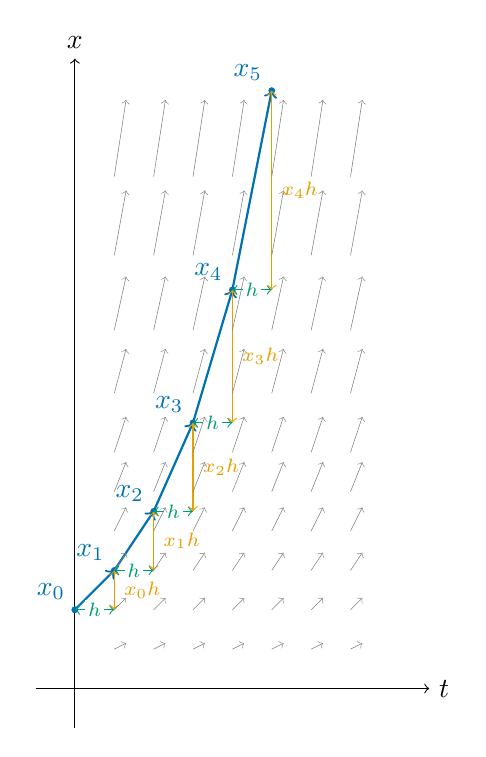
\begin{tikzpicture}

  % Axes
  \draw[->] (-0.5,0) -- (4.5,0) node[right] {$t$};
  \draw[->] (0,-0.5) -- (0,8) node[above] {$x$};

  % Parameters
  \def\xstart{1.0}
  \def\tstart{0}
  \def\h{0.5}
  \def\nsteps{5}

  % Initial values
  \pgfmathsetmacro{\x}{\xstart}
  \pgfmathsetmacro{\t}{\tstart}
  \coordinate (P0) at (\t,\x);
  \filldraw[blue] (P0) circle (1pt);
  \node[above left, blue] at (\t,\x) {$x_0$};
  \filldraw[blue] (\t,\x) circle (1pt);

  \foreach \i in {1,...,\nsteps} {
    \pgfmathsetmacro{\xnext}{\x + \h*\x}
    \pgfmathsetmacro{\tnext}{\t + \h}
    \pgfmathtruncatemacro{\ilast}{\i - 1}

    % Euler step
    \draw[blue, thick, ->] (\t,\x) -- (\tnext,\xnext);
    \filldraw[blue] (\tnext,\xnext) circle (1pt);
    \node[above left, blue] at (\tnext,\xnext) {$x_{\i}$};

    % Step size label
    \draw[green, <->] (\t,\x) -- (\tnext,\x) node[midway, fill=white, inner sep=1pt] {\scriptsize $h$};
    \draw[orange, <->] (\tnext,\x) -- (\tnext,\xnext) node[midway, right, orange] {\scriptsize $x_{\ilast} h$};

    \xdef\x{\xnext}
    \xdef\t{\tnext}
  }

  % Direction field for dx/dt = x
  \foreach \t in {0.5, 1.0, 1.5, 2.0, 2.5, 3.0, 3.5}
    \foreach \x in {0.5, 1.0, 1.5, 2.0, 2.5, 3.0, 3.75, 4.55, 5.5, 6.5} {
      \pgfmathsetmacro{\slope}{\x}
      \pgfmathsetmacro{\dt}{0.15}
      \pgfmathsetmacro{\dx}{\slope*\dt}
      \draw[gray, ->, very thin] (\t,\x) --++ (\dt,\dx);
    }


\end{tikzpicture}
\end{document}
